\documentclass[]{article}
\usepackage[style=numeric,backend=biber,sorting=none]{biblatex}
\usepackage{graphicx}
\usepackage{float}
\usepackage{pgfplots}
\addbibresource{references.bib}

% Title Page
\title{Financial Analysis Report}
\author{Mark Paveszka}


\begin{document}
\maketitle

\newpage

\begin{abstract}
\end{abstract}

\newpage

\tableofcontents

\newpage

\section{Introduction}
\paragraph{}
As a result of modern technology, the way things are done is very different compared how it was twenty years ago. Since then everything has been speeding up, including a key area of society, namely: education. In the past fifteen to twenty years several businesses emerged to make education better and easier for both students and teachers. These businesses usually try to create software artefacts to improve some aspect of the broader field. Such software artefacts are innovative learning tools and learning management systems (LMS). One of the most well-known companies in the education technology sector is Blackboard \cite{Blackboard_UK}. They provide several applications to improve the quality of teaching in higher education, business and governmental institutes. They are mostly known for Blackboard Learn \cite{Blackboard_Learn}, which is one of the most popular learning management systems currently available on the market based on data collected by Client Stat \cite{VLE-Data} and analysed by Edutechinca \cite{VLE-2020-IMG}. The aggregation of this data is shown in Figures \ref{fig:LMS-2020} and \ref{fig:LMS-2020-6-year} which depict the market share of the most popular learning management systems in four different regions. For the purpose of this analysis only the data regarding the UK will be considered. The main competitors to Blackboard are Moodle, Canvas and Brightspace. 

\begin{figure}
    \centering
    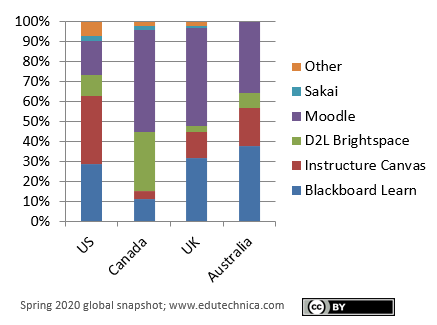
\includegraphics[width =\linewidth]{lms-vle-2020.png}
    \caption{LMS market share in 2020. \cite{VLE-2020-IMG}}
    \label{fig:LMS-2020}
\end{figure}

\begin{figure}
    \centering
    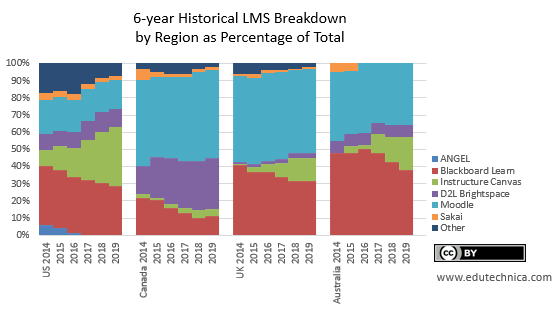
\includegraphics[width =1.2\linewidth]{lms-vle-2020-y5.png}
    \caption{6-year historical LMS data by region. \cite{VLE-2020-IMG}}
    \label{fig:LMS-2020-6-year}
\end{figure}

\paragraph{}
To obtain some data about these companies an online tool, namely Software Advice \cite{Software-Advice} was used. This tool allowed for comparisons between the companies, which provided further insight about them. The result showed that Blackboard, Canvas and Brightspace compete in the same price range, while Moodle is cheaper to use. After examining different sources it is clear that Blackboard is not a cheap software to use \cite{Blackboard-v-Moodle}, however it provides a wide variety of features for the institutions that opt to use their system.

\paragraph{}
In 2017 the education technology sector in the UK worth around £170m \cite{Government-Strategy}. This number by 2021 is expected grow to to £3.4bn which shows that there is a lot of potential in this sector. However it is worth noting that the LMS market is part of the education technology sector and even though there will be growth it might not be that significant. Also globally there is not much change \cite{VLE-2020-IMG} in the usage of these systems compared to previous years based on Edutechnica's analysis. Globally speaking there is going to be a massive growth \cite{Markets-and-Markets} even when looking at what is projected for Europe (Figure \ref{fig:Markets-LMS}). However it is worth noting that market size of Europe will only be a small portion of the global market.

\begin{figure}
    \centering
    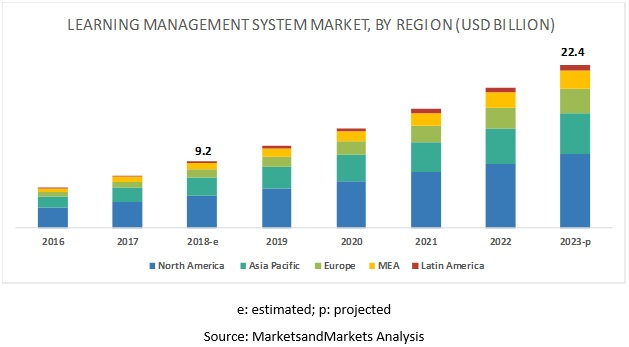
\includegraphics[width =1.2\linewidth]{learning-management-systems-market5.jpg}
    \caption{Market growth projection. \cite{Markets-and-Markets}}
    \label{fig:Markets-LMS}
\end{figure}

\newpage
\section{Financial Analysis}
\paragraph{}
In order to determine how successful Blackboard is, its financial situation needs to be examined. The following information was obtained by using FAME which is a financial database about UK based companies. To perform the analysis ratios will be used, which can be found in Table \ref{tab:Ratios-BB}. It is worth noting that Blackboard is a private company, so it is harder to find some information about it, as it does not have to publish financial statements. In Blackboard's FAME report \cite{FAME-Blackboard} the latest data entry was created in 2018. This data suggests that for the past two years the shareholder funds were decreasing somewhat. However before that this number jumped from £860k to £65m which indicates a large scale investment into the company. In 2017 the ROCE (Return on Capital Employed) ratio dropped below 0. The -14.24\% ROCE is due to the fact that the company generated a massive loss (PBT) of £-8m. This troubling trend continued in 2018, however the situations was a bit better as the ROCE value was -1.65\% which is still not negative, however it is significantly better than the 2017 one. These issues could be explained by events that happened to the company during these years. First of all Moodle ended their partnership with Blackboard \cite{Moodle-breaks-up-with-Blackboard}, which have lowered the trust in their customers. The extent this event affected the company was quite severe as they have lost their very first customers (Cornell University) in the same year \cite{Cornell-leaves-BB}. These two events combined could have easily resulted in loss of trust from other customers. It is worth noting that throughout this period, and even today Blackboard is receiving a lot of complaints for not having user friendly graphical interfaces \cite{BB-Reviews}, which could also suggest that customers were not satisfied about its products.

\paragraph{}
By taking a closer look at the Return on Shareholders Capital \ref{tab:Ratios-BB}, several conclusions can be drawn. First, the ratio values for 2018, 2017 and 2016 are the same as the ROCE values. This indicates that the total capital employed is the same as the shareholders' funds. This means that in the years mentioned, Blackboard did not have any short term loans. Secondly, the fact that this ratio was negative in the past means that Blackboard was not really popular for new investors. This is further reinforced by the fact that the Interest Cover ratio was also negative which means that Blackboard was unable to pay proper interest payments. However before 2017 this ratio was quite good, as it was 32.38\%. It must be kept in mind that Blackboard UK only had short term group loans from their parent company in the United States. Since this loan was provided by the parent company not being able to pay interest was probably not such a severe issue as if they had to pay for banks and other companies.


%TABLE
\begin{table}
\centering
\begin{tabular}{||c | c | c | c | c||} 
\hline
Ratio & 2018 & 2017 & 2016 & 2015 \\ [0.5ex] 
\hline\hline
ROCE \% & -1.65 & -14.24 & 3.39 & 96.31 \\ 
\hline
Return on shareholders capital \% & -1.65 & -14.24 & 3.39 & 99.87 \\ 
\hline
Gearing \% & 32.26 & 25.32 & 27.70 & n.s. \\ 
\hline
Interest Cover (x) & -7.52 & n.s. & 32.38 & 15.77 \\ 
\hline
Current Ratio (x) & 0.97 & 0.64 & 0.79 & 0.36	 \\ 
\hline
Quick Ratio (x) & 0.97 & 0.64 & 0.79 & 0.36 \\ 
\hline
Profit Margin \% & -2.77 & -27.08 & 5.95 & 6.33 \\ 
\hline
\end{tabular}
\caption{Ratios for Blackboard (UK) Limited from 2018 to 2015 \cite{FAME-Blackboard}}
\label{tab:Ratios-BB}
\end{table}


\paragraph{}
By looking at the quick ratio and the current ratio of the past years it is clear that they are equal. This means that there is no significant inventory that Blackboard has, which is expected since they are a selling software artefacts instead. The quick ratio measures the liquidity of a company and since there is no change to the current ratio in this case, Blackboard is probably not very good in this sense. Comparing the values of both the quick and the current ratio to the education services average values \cite{Ready-Ratios-Education} visible in Table \ref{tab:Ratios-EDSec} we can conclude several things. First that in all the years examined the current ratio remained significantly under the industry average which means that indicates higher risk of distress \cite{Investopedia-Current}. Moreover the ratio always stayed below 0 which indicates that if all of the short term obligations were due at the same time, the company would not have enough capital on hand to pay them back. The quick ratio followed the trend of remaining below average from 2015 to 2017. However in 2018 the value of the ratio (0.97) surpassed the industry average (0.86). Since the current and quick ratios were the same, they measure the same aspect of the company. Everything said for the current ratio is also true for the quick ratio. This fact also reinforces the fact that investors were not drawn to the company as they have feared that it won't be able to pay back its liabilities towards them.

\paragraph{}
By taking a look at the gearing ratio it can be concluded that there is definitely more shareholder funding in the company than long and short term loans. The gearing ratio values can be considered acceptable and good between 25\% and 50\% \cite{Investopedia-Gearing}. Based on this information Blackboard's gearing ratios in the years between 2018 and 2016 were in the acceptable range, however it was always on the lower side, rather than the upper. Even though the gearing ratio was in the optimal range, the fact that the company did not generate profits in its last two operating years can mean that the debtors would not want to give loans as it is questionable if the company can actually repay the existing debts. Also the fact there is no inventory based on the quick and current ratios, which means that there is no way for the company to quickly gain money to repay liabilities. This probably even further reduces the debtors will to provide loans for the company.


%TABLE
\begin{table}
\centering
\begin{tabular}{||c | c | c | c | c||} 
\hline
Ratio & 2018 & 2017 & 2016 & 2015 \\ [0.5ex] 
\hline\hline
Current Ratio (x) & 1.05 & 1.50 & 1.53 & 1.34 \\ 
\hline
Quick Ratio (x) & 0.86 & 1.23 & 1.24 & 1.34 \\ 
\hline
\end{tabular}
\caption{Average ratio values for Education Services sector from 2018 to 2015 \cite{Ready-Ratios-Education}}
\label{tab:Ratios-EDSec}
\end{table}


\paragraph{}
Based on the profit margins (PBT / Turnover) Blackboard was doing well during the 2015 and 2016 (Figure \ref{fig:BB-Profit-Margin}), as they respective profit margins were both above 5\%. However, there is a massive drop in 2017, which is due to the fact that the company generated an £8m loss. It is also clear that regardless off this loss Blackboard is getting better, since their profit margin in 2018 was almost 10 times better than the year before. But even with that increase in performance they still generated loss, as their profit margin shows. 

\begin{figure}
    \centering
    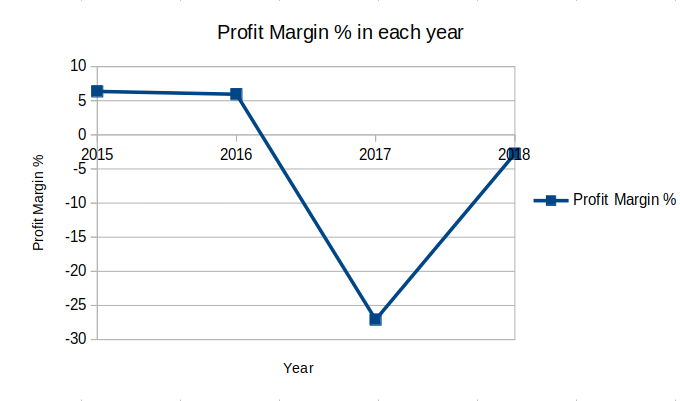
\includegraphics[width =1.2\linewidth]{profit margin.png}
    \caption{Blackboard's historical profit margin data based on FAME \cite{FAME-Blackboard}}
    \label{fig:BB-Profit-Margin}
\end{figure}

%TABLE
\begin{table}
\centering
\begin{tabular}{||c | c | c | c||} 
\hline
Ratio & 2018 & 2017 & 2015 \\ [0.5ex] 
\hline\hline
Current Ratio (x) & 1.08 & 1.09 & 1.07 \\ 
\hline
Quick Ratio (x) & 1.08 & 1.09 & 1.07 \\ 
\hline
Gearing \% & 243.33 & 2.90 & 238.34 \\ 
\hline
\end{tabular}
\caption{Ratio values for D2L Europe Limited from 2015, 2017 and 2018 \cite{FAME-D2L}}
\label{tab:Ratios-D2L}
\end{table}


\paragraph{}
To get a full view on Blackboard's financial status it is crucial to analyse other companies as well in the same sector. The companies behind Blackboard Learn's competitors will be analysed. These companies are Instructure Global Limited \cite{FAME-Instructure} and D2L Europe Limited \cite{FAME-D2L}. The latter company did not release an in-depth report, therefore only some ratios are available. Only the quick, current and gearing ratios are available for years 2015, 2017 and 2018, which can be seen in Table \ref{tab:Ratios-D2L}. Since this is also a company that produces software artefacts it was expected that the quick and current ratios will be equal. Based on the data, this company was in a better financial situation than Blackboard UK in the past couple of years as they had capital on hand to pay off their current liabilities in each year. On Figure \ref{fig:LMS-2020-6-year} it is visible that D2L's product is slowly gaining popularity in the UK, which could explain this phenomenon. In terms of the gearing ratio D2L had major fluctuations as it was either really high, or really low. This could happen due to the fact that the company took loans. This  is still in the 300\% tolerance range, which means even when the ratio was high and the investors considered it as risky it was still a manageable risk.

%TABLE
\begin{table}
\centering
\begin{tabular}{||c | c | c | c | c||} 
\hline
Ratio & 2018 & 2017 & 2016 & 2015 \\ [0.5ex] 
\hline\hline
ROCE \% & 120.57 & 401.96 & 498.92 & -285.99 \\ 
\hline
Interest Cover (x) & -7.39 & -23.35 & -35.49 & n.s. \\ 
\hline
Current Ratio (x) & 0.87 & 0.81 & 0.51 & 0.75 \\ 
\hline
Quick Ratio (x) & 0.87 & 0.81 & 0.51 & 0.75 \\ 
\hline
Profit Margin \% & -15.34 & -53.64 & n.s. & n.s.\\ 
\hline
\end{tabular}
\caption{Ratio values for Instructure Global Limited from 2015, 2017 and 2018 \cite{FAME-Instructure}}
\label{tab:Ratios-Instructure}
\end{table}

\paragraph{}
Insturcture Global Limited is the company that is creating the Canvas LMS. Currently in the industry the market share of this product is rapidly increasing, which is visible on Figure \ref{fig:LMS-2020-6-year}. This process is reflected in the ratios as well (Table \ref{tab:Ratios-Instructure}. Since 2016 Instructure's ROCE ratio is quite high, over 100\% which means that the return is much greater than the capital employed for operating. The fact that this platorm is gaining popularity can also explain why Blackboard hs been struggling with finances in the past years. In terms of interest cover rates Blackboard and Instructure is very close to each other, however while Blackboard's values are decresing, Instructure's are increasing. By comparing the rest of the data it can be said that Instructure is currently in a better situation as it is more desirable for investors than Blackboard, mostly because the latter lost a lot of market in the past couple of years. 

\newpage

\section{Change to the product}

\paragraph{}
\newpage



\printbibliography{}

\end{document}          
